\documentclass[12pt,a4paper]{report}
\usepackage{graphicx}
\usepackage{eqnarray,amsmath}
\graphicspath{{./figures/}}
\usepackage{cite}
\usepackage{amsmath}
\usepackage{amssymb}
\usepackage{graphicx}
\usepackage{float}
\usepackage{caption}
\usepackage{subcaption}
\usepackage{color}
\usepackage{url}
\usepackage[titletoc,title]{appendix}

\usepackage{multirow}
%\usepackage{subfig}
\usepackage{epstopdf}
%\usepackage[ngerman]{babel}
%\usepackage{subequations}
\usepackage[left=25.4mm, right=25.4mm,top=25.4mm,bottom=25.4mm]{geometry}
\date{}
	
	
%	\makeatletter
%	\newenvironment{varsubequations}[1]
%	{%
%		\addtocounter{equation}{-1}%
%	\begin{subequations}
%			\renewcommand{\theparentequation}{#1}%
%			\def\@currentlabel{#1}%
%		}
%		{%
%		\end{subequations}\ignorespacesafterend
%	}
%	\makeatother
	
	
	\begin{document}
		
		\begin{titlepage}
				\begin{center}
				\vspace*{0.5cm}
				
				\Huge
				\textbf{Project Title}
				
				\vspace{0.5cm}
				\LARGE
				
					B.Tech/M.Tech Category Project Report\\
									\vspace{0.5cm}
					\textit{Submitted in partial fulfillment of\\
						the requirements for the award of the degree\\
						of\\}
					\text{Master of Technology/ Bachelors}\\
							in\\
							Department of Computer Science and Engineering\\
						
				%\vspace{0.5cm}
				by\\
				\textbf{Student Name}
				\text{(Roll Number: <2K15/CSE/16>)}
				
				
				\textit{under the guidance of}\\
				\LARGE
				\textbf{Supervisor}\\
				\Large
				Supervisor Designation\\
				Department of Computer Science and Engineering
				
				\vfill
				
				
				\vspace{0.1cm}
				
				%
\includegraphics[width=0.3 height =0.7\textwidth]{DTULOGO.jpg}
				\begin{center}
												
\includegraphics[scale=0.7]{DTULOGO.jpg}

				\end{center}

				
				\normalsize
				DEPTT. OF COMPUTER SCIENCE AND ENGINEERING\\
				DELHI TECHNOLOGICAL UNIVERSITY,DELHI\\
				<MONTH> <YEAR>
				
			\end{center}
		\end{titlepage}
		
		\pagebreak
		
		
		\newpage
		\setcounter{page}{1}
		\pagenumbering{roman}
		\pagestyle{plain}
		

		
\clearpage
	   
\begin{center}
	{\large \bf CERTIFICATE}
	\end{center}

This is to certify that Project Report entitled { \bf 
Project Title} submitted by <Student Name> (<Roll Number>) for partial fulfillment of the requirement for the award of degree <Master/Bachelors Of Technology> (Computer Science and Engineering) is a record of the candidate work carried out by her under my supervision.\\ \\ \\ \\ \\
<Supervisor>\\
<Designation>\\								  	    
Project Guide\\
Department of Computer Science and Engineering \\
Delhi Technological University

\clearpage
\begin{center}
	{\large \bf DECLARATION}
\end{center}
I hereby declare that the <Report> work entitled { \bf <Title>} which is being submitted to Delhi Technological University, in partial fulfillment of requirements for the award of degree of Master/Bachelor Of Technology(Computer Science and Engineering) is a bonafide report of M.Tech/B.Tech Thesis carried out by me. The material contained in the report has not been submitted to any university or institution for the award of any degree.\\ \\
<Student name>\\ 
<Student Roll number>

\clearpage
\begin{center}
{\large \bf ACKNOWLEDGEMENT}
\end{center}
I would like to express my gratitude and appreciation to all those who gave me the support to complete this project.\\ 
A special thanks to my mentor and project guide, {\bf Supervisor }, ... \\ \\ \\
\vspace{0.7in}
(Student Name) \hspace{1in}
\clearpage
\begin{center}
	{\large \bf ABSTRACT}
	\end{center}
This project aims to ...
\clearpage
\newpage
\tableofcontents

\newpage
\listoffigures

\newpage
\setcounter{page}{1}
\pagenumbering{arabic}
\pagestyle{plain}

\pagebreak

\chapter{Introduction}

\section{Overview}
\clearpage
\section{Motivation}

\clearpage

\section{Problem Statement}
The main objective of this research work is to improve ..
%Discrete event simulation allows the user to define the system, evaluate service and arrival patterns, and various other dimensions of the system.
%The simulation helps to replicate the actual behavior of the system in reality, and the results
%are evaluated to determine system performance.

\chapter{Literature Review}
Different sections to highlight the background related information
\section{Figures}
Sample Figure \ref{fig1}.
\begin{figure}[h!]
	\begin{center}
		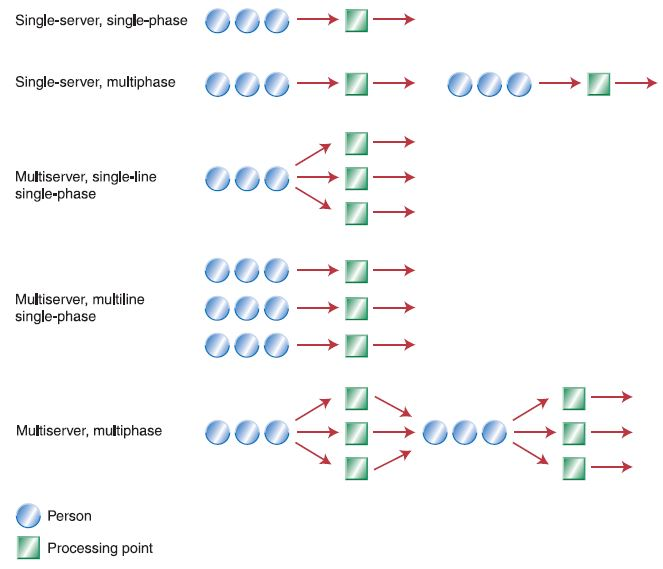
\includegraphics[scale=0.6]{servers.JPG}
		\caption{Examples of various Queuing systems}
		\label{fig1}
	\end{center}
\end{figure}

\section{Equations}
Sample Equations...
 We can write L\textsubscript q as given below.\\\\
\[L_q= \sum_{n=c}^{ \infty } (n-c)P_n \]
\\
To determine Lq, substitute j=n-c or n=c+j in the above equation as shown below.
\[L_q= \sum_{n=c}^{ \infty } (n-c)P_n \]\\
	Pc+j can be written as,
\[P_{c+j}= \left(\frac{ \lambda }{ \mu }+\frac{ \lambda  }{2\mu}+....+\frac{ \lambda  }{c \mu} \right)\left (\frac{ \lambda  }{c\mu} \right) ^{j} P_0 \]

\pagebreak
which can be again written as,\\
\[ =\left ({\frac{\rho ^{c+1}}{c!Xc^{j}}}  \right )
X P_0 X \frac{\partial \left(\sum_{j=0}^\infty\left ( \frac{\rho }{c} \right )^{j} \right)}{\partial \left ( \frac{\rho }{c} \right )}\]\\
\[ = \left ({\frac{\rho ^{c+1}}{c! X c^{j}}}  \right )
X P_0 X \frac{\partial \left ( \frac{1}{1 - \frac{\rho }{c}} \right )}{\partial \left ( \frac{\rho }{c} \right )}\]\\
\[L_q = \left ( \frac{\rho ^{c+1}}{(c-1)!(c-\rho )^{2}} \right )P_0 \]

After determining L\textsubscript q , using Little’s law we can determine the waiting time in the queue W\textsubscript q as shown below.\\\\
\[W_q= \frac {L_q}{ \lambda } \]

Patients waiting in the service system will be sum of W\textsubscript q and service time.\\\\
\[ W=W_q+ \frac{1}{\mu} \]

The number of patients in the service system,\\\\
\[ L=\lambda W  \quad (Using \quad Little's \quad law) \]
\[ = \lambda W_q+\frac{\lambda}{\mu}\]

\pagebreak
\subsection{Subsection name}
The Poisson distribution \cite{feng2016steady} is a discrete event probability distribution that keeps track of no. of events that occurring randomly for a given period of time or space.\\
If say X = The no. of events occurring in the system in a given period,\\
\section{Electronic Health Records (EHR)}
\subsection{HL7}
\subsubsection{FHIR Architecture and Implementation}
Figure for architecture \ref{figfhir}
\begin{figure}[h!]
	\begin{center}
		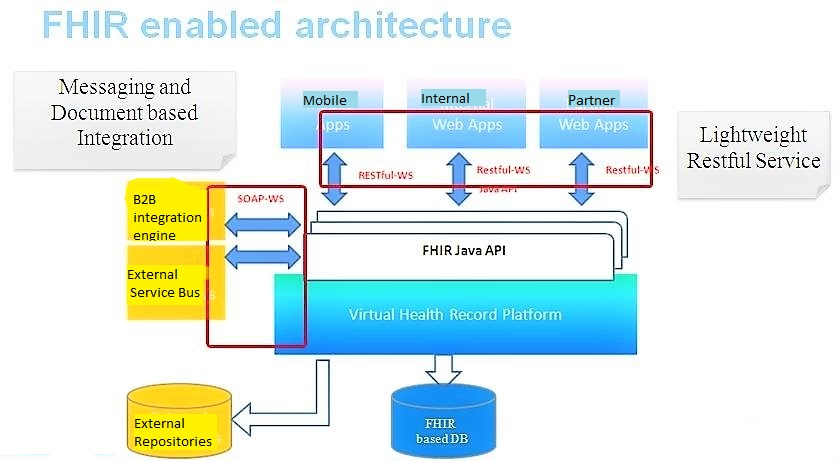
\includegraphics[scale=0.7]{arch.jpeg}
		\caption{FHIR Enabled Architecture} \cite{small}
		\label{figfhir}
	\end{center}
\end{figure}
\clearpage
{\bf Sample FHIR data}\\\\
{\bf Observation Example}


\clearpage

\subsubsection{Semantic Interoperability}
Check citations
M.Fam et al. in their research work \cite{fan2016smart} have taken Wuhan Smart Health as a case to describe
the typical smart health construction model in big city of central China. They have described one network dedicated network for smart health and common platform for all services, i.e. a smart health information platform, which is the core of the whole project. It contains the municipal
and district information platforms, and three kinds of
smart health cloud services (healthcare, public health,
medical management). The former needs cloud computing
and cloud storage technology; the latter is based on
the EMR and EHR database. However, in their Wuhan smart health care system nowhere they have considered portability and interoperability of electronic health records.\\

Nikakhtar et al. \cite{nikakhtar2015social} in their research work have used

\chapter{Proposed Work}
\section{Present workflow of system}
\begin{figure}[h!]
	\begin{center}
		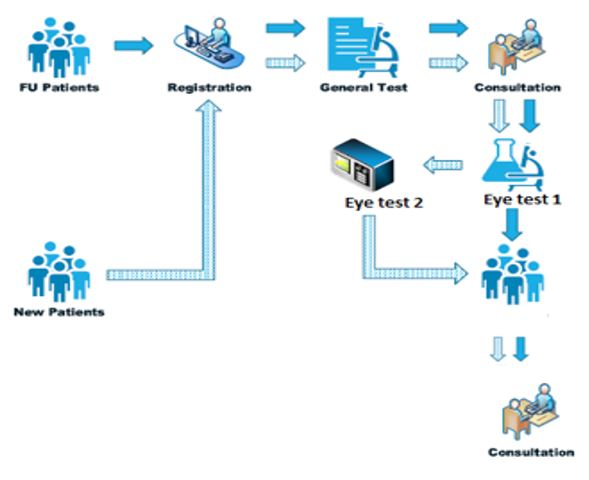
\includegraphics[scale=1]{flow.JPG}
		\caption{General flow of patients in department}
	\end{center}
\end{figure}

\pagebreak
\section{Proposed workflow of system/ Proposed Algorithm/ System}
\clearpage
\begin{figure}[h!]
	\begin{center}
		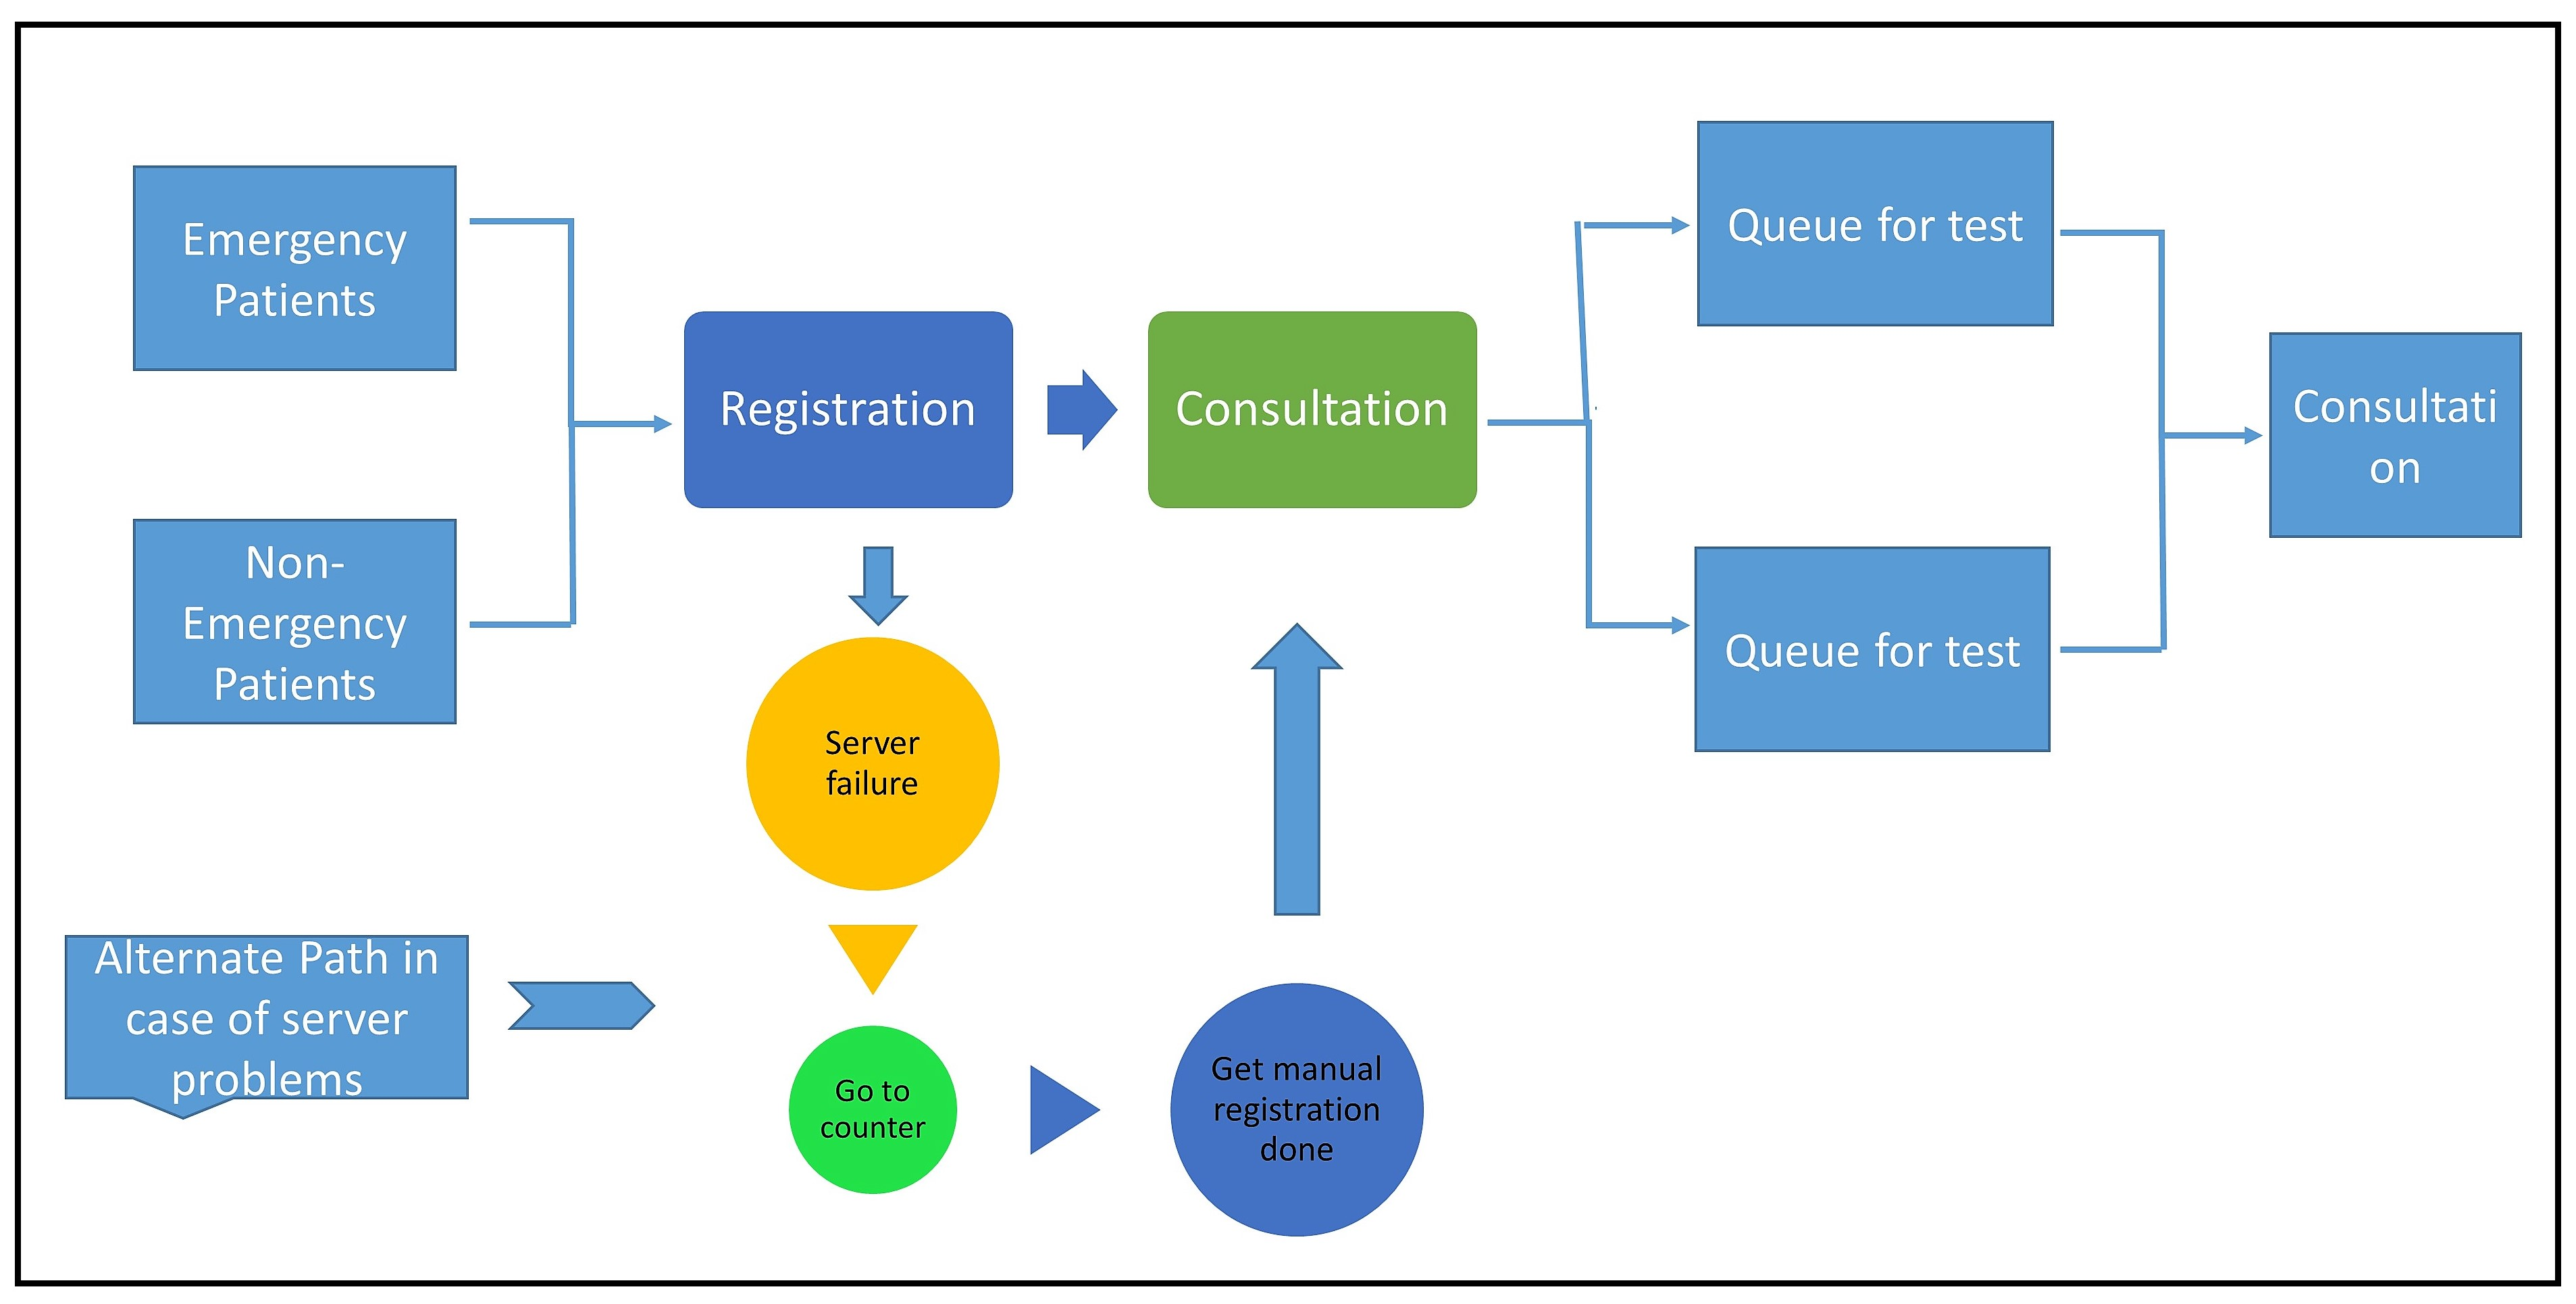
\includegraphics[scale=0.5]{final.jpg}
		\caption{Proposed work flow of department}
	\end{center}
\end{figure}
{\bf Main components of our research work:-}
\subsection{Smart Registration process}

\subsection{Portable Health Records}

\chapter{Experimental Results}

\section{Experimental Environment}

\begin{table}[h]
\centering
\caption{Simulation Environment statistics}
\label{my-label}
\begin{tabular}{|l|l|l|}
\hline
                &Parameter     & Value                \\ \hline
1.   & Simulation duration   & 4 hours                  \\ \hline
2.   & Number of patients per day   &200                  \\ \hline
3.   & Arrival Rate   &60 arrivals per hour                 \\ \hline
4.   & Probability of kiosk failure       & 1/100       \\ \hline
5.   & Probability of server outage       & 1/50                \\ \hline

\end{tabular}
\end{table}


\section{Simulation of present system}
\begin{figure}[h!]
	\begin{center}
		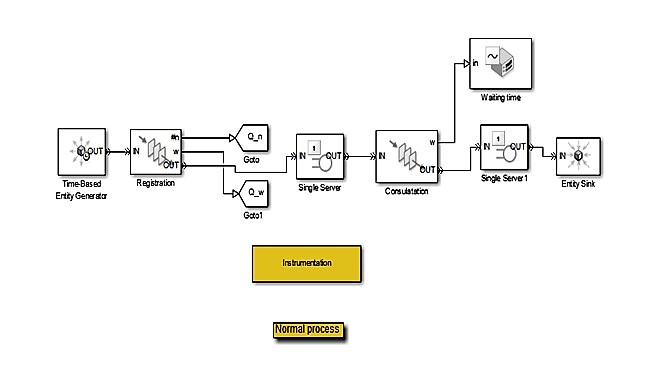
\includegraphics[scale=1]{pr2.jpg}
		\caption{Screenshot:Present workflow of department}
	\end{center}
\end{figure}
\begin{figure}[h!]
	\begin{center}
		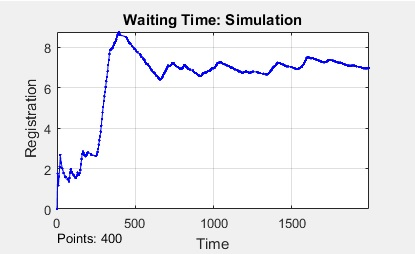
\includegraphics[scale=1.1]{exp2.jpg}
		\caption{Waiting time for registration process}
	\end{center}
\end{figure}
\begin{figure}[h!]
	\begin{center}
		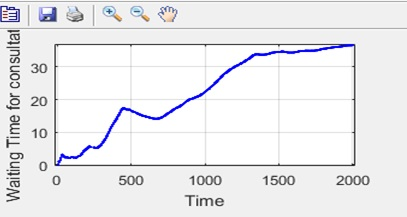
\includegraphics[scale=1.1]{exp1.jpg}
		\caption{Waiting time for consultant}
	\end{center}
\end{figure}
\clearpage
\section{Simulation of proposed system}
\begin{figure}[h!]
	\begin{center}
		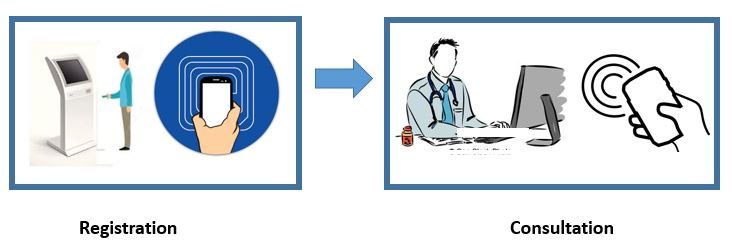
\includegraphics[scale=0.6]{propo.jpg}
		\caption{Proposed system with portable electronic health records}
	\end{center}
\end{figure}
TAble:
\begin{table}[]
\centering
\caption{Statistics for specialty clinics \cite{rpc}}
\label{my-label}
\begin{tabular}{|l|l|l|l|l|}
\hline
    & Specialty Clinic           & New cases & Old Cases & Total  \\ \hline
1.   & Cornea Clinic              & 5959      & 11524     & 17483  \\ \hline
2.  & Lens Clinic                & 825       & 1955      & 2780   \\ \hline
3.   & Uvea Clinic                & 1079      & 3667      & 4746   \\ \hline
4.   & Contact Lens Clinic        & 985       & 2239      & 3224   \\ \hline
5.   & Glaucoma Clinic            & 3759      & 11195     & 14954  \\ \hline
6.   & Oculoplasty Clinic         & 3305      & 2493      & 5798   \\ \hline
7.   & Paed. Ophthalmology Clinic & 418       & 36        & 454    \\ \hline
8.   & Retina Clinic              & 3883      & 4904      & 8787   \\ \hline
9.   & Neuro-Ophthalmology Clinic & 2584      & 2328      & 4912   \\ \hline
10. & Vitreo retinal Clinic      & 2478      & 2282      & 4760   \\ \hline
11. & ROP                        & 830       & 1124      & 1954   \\ \hline
12.  & Ocular Oncology Clinic     & 378       & 1329      & 1707   \\ \hline
13.  & Low visual Aid             & 2798      & 464       & 3262   \\ \hline
14.  & Orthoptic Clinic           & 2211      & 21265     & 23476  \\ \hline
15.  & Squint Clinic              & 5205      & 19982     & 25187  \\ \hline
16.  & Refraction                 & 40644     & 40644     & 40644  \\ \hline
    & Total Cases                & 36697     & 127431    & 164128 \\ \hline
\end{tabular}
\end{table}
\begin{table}[]
\centering
\caption{Total Cases in Dr. Rajendra Prasad Centre for Ophthalmic Sciences at AIIMS \cite{rpc}}
\label{my-label}
\begin{tabular}{|l|l|r|l|l|}
\hline
\multicolumn{2}{|c|}{} & New Cases & Old Cases              & Total  \\ \hline
1.   & General O.P.D.  & 152455   & 99349                  & 251804 \\ \hline
2.   & Emergency       & 8799     & \multicolumn{1}{c|}{-} & 8799   \\ \hline
     & Total Cases     & 161254   & 99349                  & 260603 \\ \hline
\end{tabular}
\end{table}

\clearpage
\label{whatever}
%\input{appendixA} % filename in curly brackets
%\chapter{Name of Appendix B}
%\label{whatever}
%\input{appendixB} % filename in curly brackets**
\clearpage
Please check correct format for articles, proceedings and url.
Captilalisation of alphabets in titles, last access date in url
\bibliographystyle{IEEEtran}
\bibliography{dtucse} 

\end{document}}
